\documentclass[12pt]{article}
\usepackage{amsmath}
\usepackage{placeins} 
\usepackage{graphicx}
\usepackage{float}

\begin{document}
 
%******************%
% START TILTE PAGE %
%******************%

\thispagestyle{empty}
\begin{center}
\begin{minipage}{\linewidth}
    \centering
%University logo
    
\includegraphics[width=0.5\linewidth]{UP.jpg}
    %\rule{0.4\linewidth}{0.15\linewidth}\par
    \vspace{1cm}
%Thesis title
    {\uppercase{\Large \\ Prioritized Foraging using \\ Robot Swarms \par}}
    \vspace{1cm}
\end{minipage}

%Author's name
    {\Large \begin{minipage}{\linewidth}	
    			Student number \\ 10153285 \\
    			Contact number \\ 082 323 3108 \\
			\end{minipage} 
	\par }

\begin{minipage}{\linewidth}
	\centering
    \vspace{1cm}
%Degree
    {\Large University of Pretoria \\ Department of Computer Science \\ COS 700 Research Proposal \par}
    \vspace{1cm}
%Date
    {\Large 27/04/2015}
\end{minipage}
\end{center}
\clearpage

%************%
%* Abstract *%
%************%
\begin{abstract}
This empirical study aims to improve on the problem of prioritized foraging by using robotic swarms. The attempt will introducing clustering during the foraging process to improve the over all performance of foraging. The paper focuses on swarm intelligence in corporation with swarm robotics through using social insect colonies behavior as the work force. Previous work has shown that ant cemetery clustering and honey bee foraging algorithms are successful in collaboration for this study. Honey bee foraging is used for the ability to adapt to  dynamic environment and the ant cemetery clustering not requiring peer to peer communication or pheromone deposits. These algorithms are highly successful at path finding, grouping and retrieval of prioritized object, this directly correlates to the optimization goal of the paper.
\end{abstract}

%****************%
%* Introduction *%
%****************%
\section{Introduction}

\par{The gold mining industry has grown in complexity where deep shaft mining is required to access richer gold deposits. At these depths in particular to conditions for humans has become impractical, highly expensive \& dangerous. To retrieve these gold deposits using Swarm Robotics can be seen as more efficient, safer \& at lower maintenance costs. These is swarm robotics model is made possible by using Swarm Intelligence.}
\\
\par{Swarm Intelligence (SI) is a broad field of algorithms modeled after animal \& insect behavior in nature \cite{SI}. This paper will focus on the algorithms simulated after ant cemetery clustering and of honey bee foraging. This algorithm is a colony based eco-systems used as priority is foraging. This is defined as search and retrieve process from the environment to a collection point \cite{Forage-09}. As for the other Ant cemetery clustering by \cite{Lumer-Faieta} where ants cluster their dead based on the object density in their surrounding area.}
\\
\par{Swarm robotics uses an amount of robots with simplistic abilities working together as a collaborative entity \cite{Robots-Dorigo} as it is designed by SI. It can be seen as an entity with mechanisms where each is a specific behavior where together these entities collaborate in a swarm. These robots are build \& designed around the idea of self-organized social systems where the dynamic mechanics drive the entire system towards a goal \cite{SI}.}
\\
\par{The research methodology to be followed and the process to complete the study. A literature review of background research relevant to the topic helping to get a better understanding and show the knowledge obtained during preparation for the paper. The project plan showing the sub-section of the project and project projection from start to submission. Also to show the study timely and no previous research has been done on this exact topic before.}
\\
\par{I will follow up on a publication by Jade Abbott \cite{Jade-2014} around Prioritized foraging looking at multiple foraging methods. In her study the methods where tested against each other to determine their efficiency in different environment simulations. From the study the honey bee algorithm has performed best under most situations, and indicates that it would perform best in dynamic environments. This study will introduce the property of clustering before and during foraging to improve the foraging process due to prioritized objects being in a closer vicinity of each other.}

%*********************%
%* Problem Statement *%
%*********************%
\section{Problem Statement}

\par{Prioritized Foraging using Robot Swarms is required by the mining industry when looking at deep mining where humans can't retrieve the gold ore after blasting has occurred. This is due to the reduced amount of oxygen, increased levels of sulfur dioxide and nitrogen dioxide also over whelming heat. These problem contribute to increasing operation cost and unacceptable working conditions. All of this is irrelevant when looking at using robots to retrieve the gold and working prolonged hours.} 
\\
\par{The empirical study will simulate the behavior which will be programmed on a swarm of robots to cluster and forage the gold and rubble out of the mine. The foraging aspect will come in with retrieving the objects. Clustering to the grouping of objects to simplify the foraging process and prioritization to the gold and rubble objects respectively. This work research foraging and clustering but limits itself to only Ant Cemetery Clustering and Honey Bee Foraging, to keep with the SI model applicable to robots and by results of the standing study \cite{Jade-2014}.}
\\
\par{I am aiming to determine how clustering of the prioritized items will improve on the foraging process, division of labor will be introduced where robots switch between clustering and foraging as needed to improve performance. This empirical study will prove that deep mining can be undertaken with the use of robots when physical simulations have been tested. No other study has been done on concurrent clustering of the prioritized object while foraging takes place to improve feasibility and performance.}

%************************%
%* Research methodology *%
%************************%
\section{Methodology}

\par{The proposed paper will consist of Prototyping and Simulations to be discussed in section 3.1 and 3.2.}

\subsection{Prototypes}

\par{A prototype will be developed combining the algorithms being used to be able to run the simulations. It will consist of the following components of development:
\begin{itemize}
	\item 	A controller which controls all the simulations to be run with all the 					variations of configurations.
	\item 	Honey bee foraging mechanism module, where each robot entity explores 					the search space for the prioritized object to carry them out the 						collection point as a bee would honey.
	\item 	Ant cemetery clustering mechanism module, where each robot entity when 					discovering a prioritized object it has to cluster it as ant would his 					dead.
	\item 	Division of labor module controlling the decision process where each 					robot entity must decide between the two mechanic modules.
\end{itemize}
}

\subsection{Simulations}

\par{The simulations will test this prototype on a 2D grid that will simulate the environment where the robots might find themselves. The set of configurations to be tested are drawn from possible situations described in \cite{Jade-2014}:}
\begin{itemize}
	\item 	Scattering layout of how the prioritized items are scattered around the search space.
	\item	Grid size variation the search space and increasing complexity of the clustering \& foraging and run time.
	\item	Grid coverage percentage of prioritized items over the open search spaces.
	\item	Ratio of the amount of gold objects versus that of the rubble.
	\item	Priority of foraging gold over rubble if in a close proximity.
	\item	Number of robot entities in the search space.
\end{itemize} 
\par{Each configuration simulation will be test 30 times for sufficiently comparable results. These simulations will each run on a concurrent thread increasing multi-thread support. The simulations will be test on a Amazon compute module to improve testing times due to the high concurrency provided.}

%*******************%
%* Research review *%
%*******************%
\section{Literature Survey}
\par{The study will be based around a paper by Abbott \cite{Jade-2014}, various foraging methods where tested against one another: naive foraging, honey ant \& desert ant. This study will build on previous work by taking the proven best foraging algorithm and add a clustering process. It can be seen as a dynamic system where clustering and foraging are inter changed by each robot as the need occurs. The require research fields to complete this study is discussed in detail in the following sub-sections.}

\subsection{Swarm Intelligence / Robotics}
\par{Swarm Intelligence (SI) as defined by Gerando Beni \cite{Beni-Robot} it is 'A group of non-intelligent robots ("machines") capable of universal material computation'. He further stated that SI can be divided in to sets, where ACO and PSO algorithms are more suited to swarm automata due to its pattern analysis behavior, also termites behavior of structure building is suited to intelligent robot behavior. The foraging and clustering behavior used is more suited for swarm robots due to it does not follow any pattern analysis but more of an opportunistic behavior by its mechanical ability.}
\\
\par{Swarm-based robotics is defined by Bonabeau \textit{et al} \cite{Robot-Swarm} that it may be able to perform tasks without needing a explicit representation of the environment. These self organized social insects use a communication method call stigmergy \cite{Robot-Swarm}, it can be in a form of direct and in-direct communication. Where direct is in the form of physical information exchange \& in-direct by means of environment changes.
\\
\par{Stigmergy will be used as direct and in-direct by this study in the following ways:}
\begin{itemize}
	\item Direct:
			The honey bee broadcasts a foraging site by dancing when it arrives at 					the	hive, this dance indicates the direction the other bees should follow to the site. 
	\item In-direct:
			Ant cemetery clustering where each ant exams the environment to determine if an object should be picked up or dropped while clustering.
\end{itemize}
\par{These communication methods will discussed in the expanded section of clustering and foraging.}

\subsection{Clustering}
\par{Ant colony clustering will be used due to the application where it needs to be develop for a large amount of cooperative robots. This possible by the social ability of ant and how they work together to achieve a goal. A basic ant colony clustering model was inspired by Chrètien \cite{L-Chretien} about the \textit{Lasius niger ants} and develop by Deneubourg \cite{RobotAnt} as the first algorithm. This study will only focus on a improved ant cemetery algorithm by Lumer \& Faieta \cite{Lumer-Faieta}.}
\\
\par{These clustering algorithms use the ant cemetery model where ant pick up died ant from a low populated area \& dropping it when its in a higher populated area or when the work load becomes to high. The algorithm aim to maximized inter-cluster distance (cluster separation) and minimize intra-cluster distance (cluster density). While performing clustering the ants will be moving around randomly in the search space monitoring a neighborhood of \( N^2 \) where N is the visual distance.}
\\
\par{The "local" population density \( \lambda(y_{a}) \) where \( i \) is the ants position at time step \( t \) and \( \gamma \) the scale of dissimilarity is given as \cite{Lumer-Faieta}:}
\[ \lambda(y_{a}) = max \left\{ 0, \frac{1}{n^2_{N}} \sum_{y_{b} \in N_{n_{N} x n_{N}}\left( i \right) } \left( 1 - \frac{d \left( y_{a}, y_{b} \right)}{\gamma} \right) \right\} \]
\par{In neighborhood \( N \) and \( n_{N} \) the sites surrounding \( i \). The constant \( \gamma \) determines is two object of priorities have to be placed together.}
\\
\par{Ants use probability to decide it a object needs to be picked up if it isn't burdaned and dropped if the amount of work exceeds the limits \cite{Lumer-Faieta}:}
\[ P_{p} \left( y_{a} \right) = \left( \frac{\gamma_{1}}{\gamma_{1} + \lambda_{y_{a}}} \right)^2 \] 

\[ P_{d} \left( y_{a} \right) = \begin{cases} 2 \lambda \left( y_{a} \right) & \mathrm{if \lambda \left( y_{a} \right) < \gamma _{2} }\\ 1 & \mathrm{if \lambda \left( y_{a} \right) \geq \gamma_{2}} \end{cases} \]

\par{These measures allows progression without any physical communication between the robots it can rely only on detection of the environment. The clustering process will not only be used as a process to improve the performance of foraging, but also as a testing condition where the search space is pre-clustered. This will especially test the ability of the division of labor to see if the ant realize it is already clustered and switch to a bee state.}

\subsection{Foraging}
\par{Honey bee foraging will be used for collecting the prioritized objects from the environment as they are clustered. The honey bee specific algorithm is used due to the results from \cite{Jade-2014} where it has shown good results in a most cases and in dynamic environments. This process was derived from a study done by Seeley \cite{T-Seeley}. There are three roles bees take during foraging:}

\begin{itemize}
	\item Scouts: Exploring the environment to find new sources of the prioritized objects. Once a source is found it return to the "hive" and broadcasts the message of the source. This message contains the direction vector to be used by the remainder bees to follow towards the source and its distance. The process is call recruiting of unemployed foragers.
	\item Unemployed foragers: Waits in the "hive" for a dance to be detected. Once the message is received it decides towards which source it will move, becoming an employed forager. 
	\item Employed foragers: Using the source information it attempts to find the prioritized objects. If it was able to find the objects it picks up an object and returns to the hive where unemployed foragers are waiting to offload it.
\end{itemize}

\par{During the scouting process the bee is constantly aware of the hives location and moves randomly through the search space until objects are found. If a source is found it moves directly as possible back to the hive to preform the dance for unemployed foragers.}
\\
\par{Scouts use density to determine the viability of a forage site as \( \mu_{t} \), this is detected within the visible distance of the robot \cite{T-Seeley}.}

\[ \mu_{t} = \frac{1}{n} \sum_{i=1}^{n}k_{i_{t}} \]

\par{Where the distance value received from the sensor of item \( t, k_{i_{t}} \) is calculated as:}

\[ k_{i_{t}} = \begin{cases} k_{i} & \text{if item \(i\) is type \(t\)}\\ 0 & \mathrm{otherwise}\end{cases} \]

\par{The following cases when non-prioritized item are foraged as from \cite{Jade-2014}:}

\begin{itemize}
	\item If no prioritized items was located within time \( f_{max} \).
	\item Non-prioritized items are foraged until the site can not be located where it switches to prioritized items.
	\item It will not communicate the location of non-prioritized objects.
\end{itemize}

\subsection{Division of labor}
\par{A colony has proven to be efficient at dividing labor between its working within the ecological system, this is done by giving a subset of tasks to each robot.
%cite 625%
%read - ants 328, 348, 558, 693, 882 bee 393, 625, 733
}
\\
\par{Multiple task selection \cite{Engel} uses a threshold vector \( \theta_{k} \) and  \( \theta_{kj} \) the stimulus threshold, where \( k \) denotes the number of worker on the task \( j \). After a specified time a robots will have a chance to select a new task, it may happen that it is the same task, the probability of the function selected is \cite{Engel}:}
\[ P_{\theta_{khj}}\left( s_{j} \right) = \frac{s_{j}^\omega}{s_{j}^\omega + \theta_{kj}^\omega} \]
\\
\par{The division of labor process has not been finalized upon of which algorithm will be used by each robot to switch between clustering and foraging. This decision will only be made if times allows for it after the other process have been thoroughly been tested and deemed completed.}


%****************%
%* Project plan *%
%****************%
\section{Project Planning}

\par{The project plan covers research, prototyping, testing, re-factoring, writing of the article \& supervisor review. These section cover the following:}
\begin{itemize}
	\item Research : \\ Read up on all the required topics starting at the that this research follows up on, then to the references of that paper and further.
	\item Prototyping / Programming : \\ Implementation of the prototype to be able to test the improvement of clustering for the foraging and division of labor between the processes.
	\item Testing / Re-factoring : \\ Running simulations of each configuration clustering and foraging. Also to implement changes required if it is necessary after a testing cycle is completed.
	\item Writing article : \\ Writing the article to be submitted of approximate 15 pages.
	\item Supervisor review \& edits : \\ The supervisor will review the article and request chances if needed.
\end{itemize}

\vspace{0.1cm}

\flushleft The project time-line is constructed as follows:

\vspace{0.2cm}

\begin{figure}[H]
	\begin{center}
		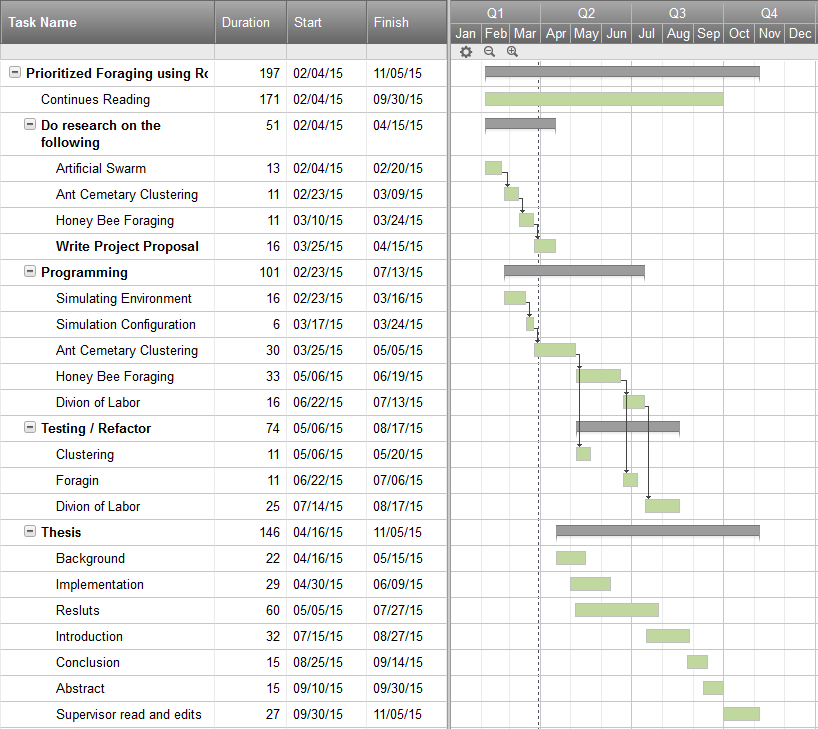
\includegraphics[width=\textwidth]{Planning.png}
	\end{center}
\end{figure}

\bibliography{reference}{}
\bibliographystyle{plain}

\end{document}
